% !TEX root =  ./main.tex

\section{Encoding of RS in GT}\label{sec:RS2GTS}

As an alternative to \BioResolve, we investigate the use of graph transformation and \GROOVE to generate the underlying LTS of a given Reaction System, on the basis of a start graph obtained by transformation from the RS specification. Because the start graph will typically include special \Entity subtype, it comes together with an additional type graph where those are specified. Depending on what one wants to analyse, the various strengths and capabilities of \GROOVE then come into play.

For instance, one possibility is to use \GROOVE's model checking capabilities to check for temporal patterns of entity generation in the transition system. Another way to proceed is to focus on a given trace and build its \emph{occurrence graph}, which contains all the rule occurrences and entity instances present in that trace --- analogous, in fact, to the way a Petri net process captures a particular behaviour. If the trace in question leads to a state in which a \Forbidden entity is present (such as the $\bang$ entity in our toy example), we can also \emph{prune} the occurrence graph, again using graph transformation, to keep only those rule occurrences and entity instances that directly contributed to the existence of the forbidden entity.

This gives rise to the tool chain depicted in \Cref{fig:chain}, the phases of which will be explained in some more detail in the remainder of this section.	

\begin{figure}
\centering
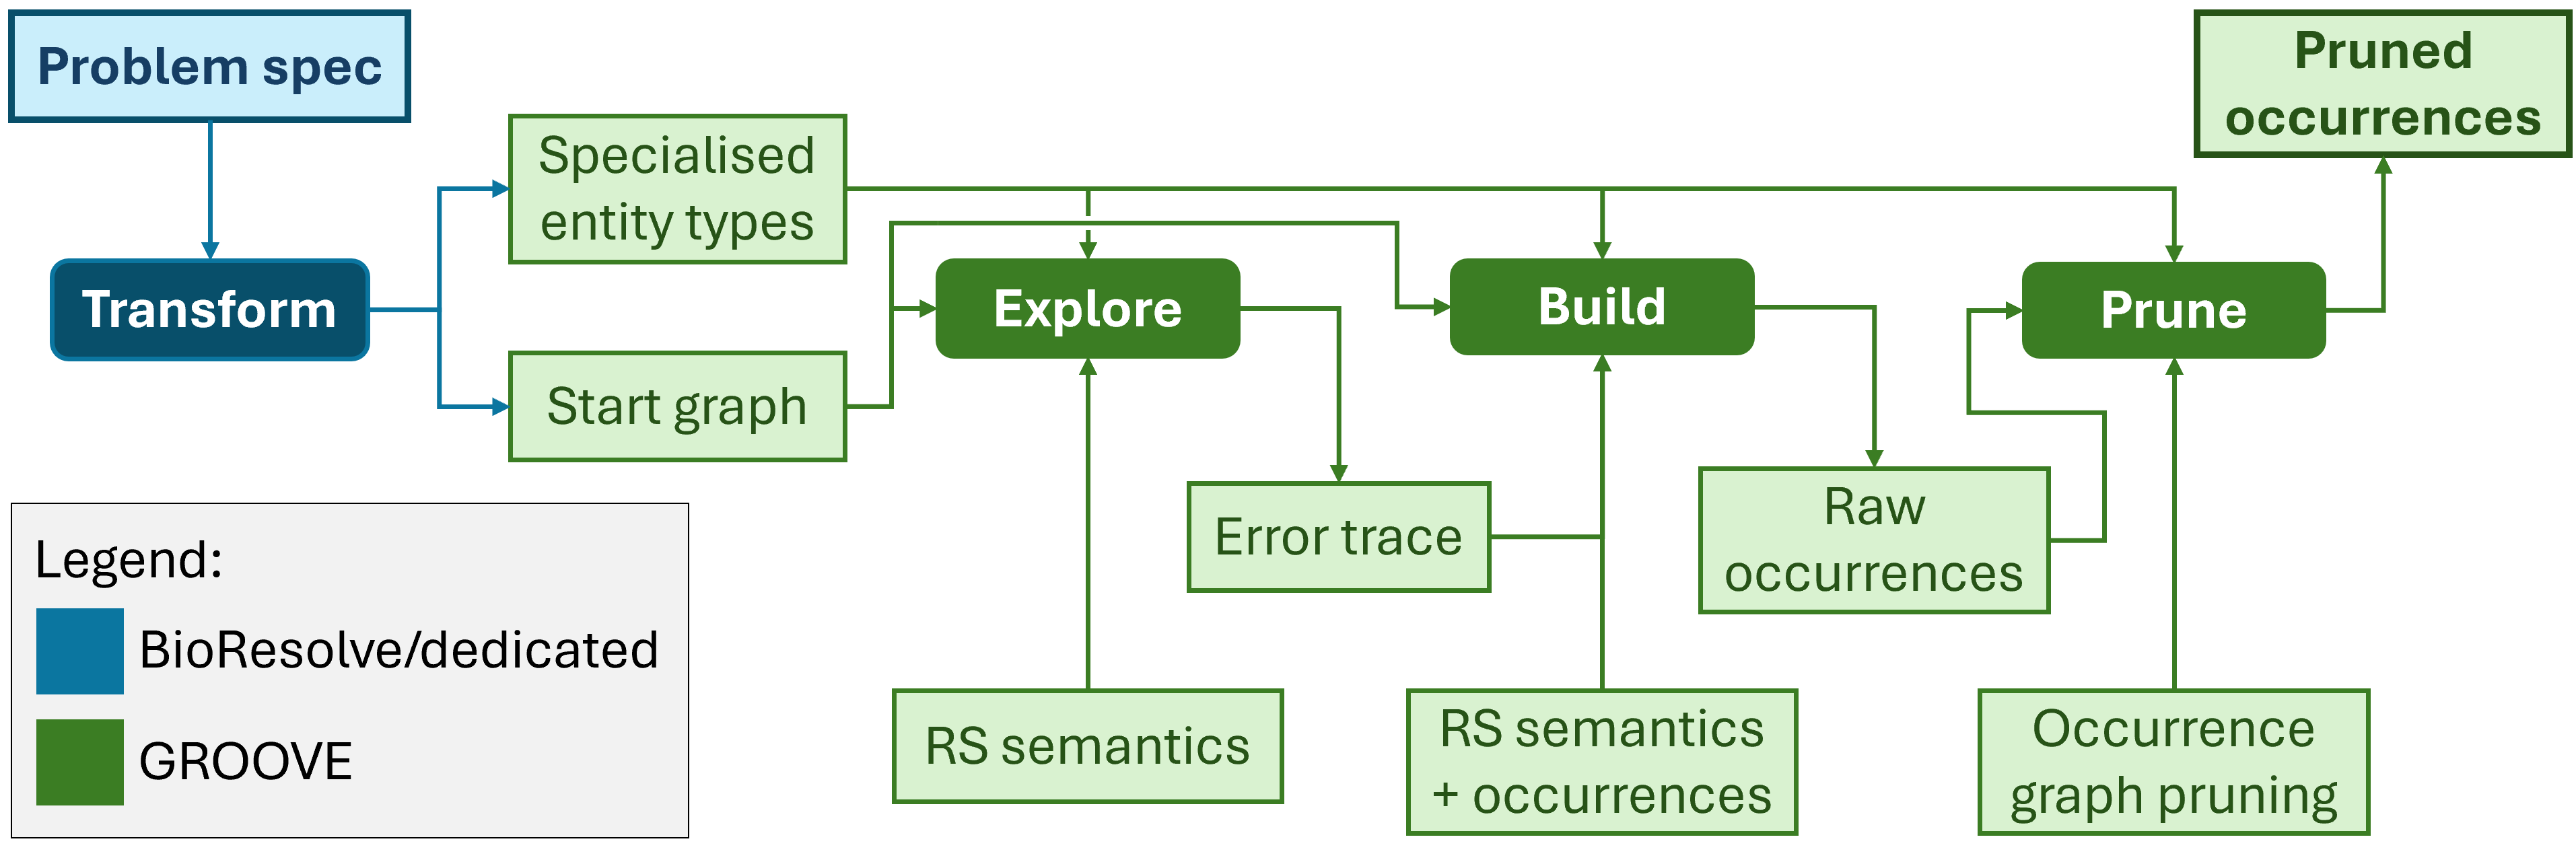
\includegraphics[scale=.27]{figs/chain}
\caption{Reaction System exploration and analysis using \GROOVE}
\label{fig:chain}
\end{figure}

\medskip\noindent\textbf{Transform.}
%
The first step is a text-to-model transformation from a problem specification in \BioResolve syntax into \GROOVE syntax. This is achieved by running the \verb=main_do(rs2gts)= directive of \BioResolve, which produces two artifacts: firstly, an additional type graph, complementary to the one shown in \Cref{fig:core-type}, which specifies subtypes of \Entity for all entities in the problem at hand (essentially for performance reasons: relying on dedicated types speeds up the matching step of \GROOVE); and secondly (more importantly) a start graph in which the entire \BioResolve system is encoded as suggested by \Cref{fig:core-type}. For the example system, the additional types as well as two self-explanatory fragments of the start graph are shown in \Cref{fig:toy}.

\begin{figure}
\centering
\subcaptionbox{Specialised entity types}{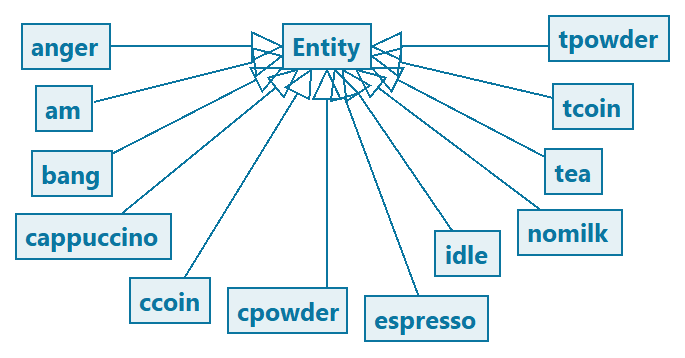
\includegraphics[scale=.2]{figs/toy-type}}
\subcaptionbox{Start graph fragment: Three reactions from $\mathsf{VM}$}{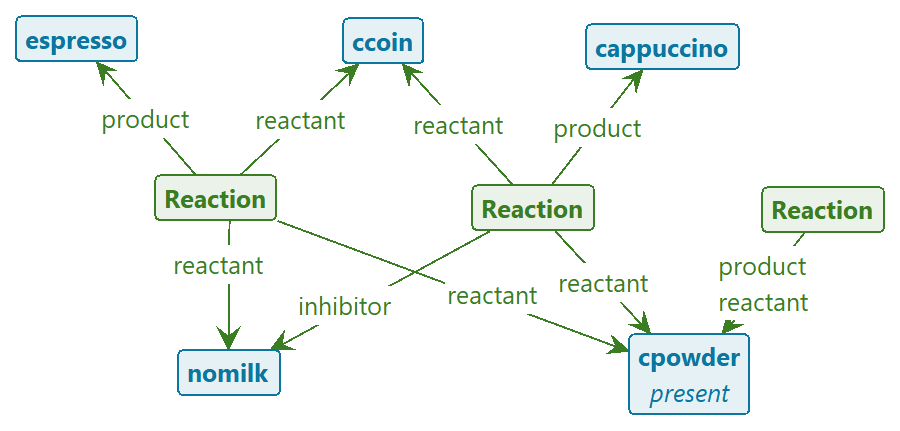
\includegraphics[scale=.2]{figs/toy-reactions}}
\subcaptionbox{Start graph fragment: The \textsf{Student} context process}{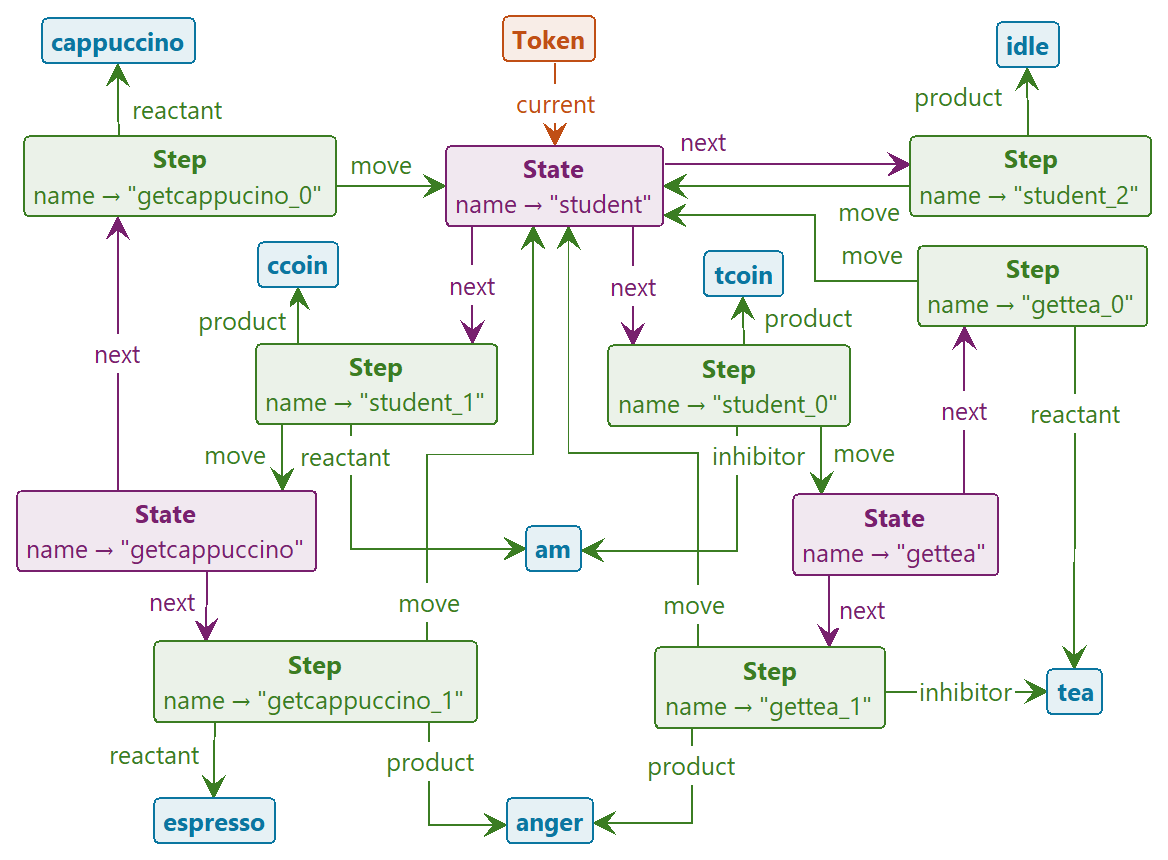
\includegraphics[scale=.2]{figs/toy-context-named}}
\caption{Graph representation of running example}
\label{fig:toy}
\end{figure}

\medskip\noindent\textbf{Explore.}
%
The dynamics of Reaction Systems is encoded as a combination of two rules, \contextR and \reactR, which are scheduled to fire in alternation. The rule \contextR encodes the simultaneous firing of all context processes (nondeterministically selecting an enabled \Step from every \State with a \Token), whereas \reactR encodes the (deterministic) simultaneous firing of all enabled \Reaction{}s, while simultaneously erasing all \Entity{}s that were not just produced. The production or erasure of an \Entity is encoded through the creation or deletion of a \present flag on a (persistent) \Entity node, \emph{not} by the creation or deletion of the node itself. In addition, to keep track of which nondeterministic choices were actually taken, the \contextR rule marks the \Step{}s that were selected with a \fired flag, which is subsequently erased by the \reactR rule. % A third rule called \firedR (actually a \emph{condition}, which in \GROOVE is a rule that does not modify the graph) checks for the occurrences of the \fired flag and so exposes the names of the \Rule{}s that have fired in the transition system.

\begin{figure}
\centering
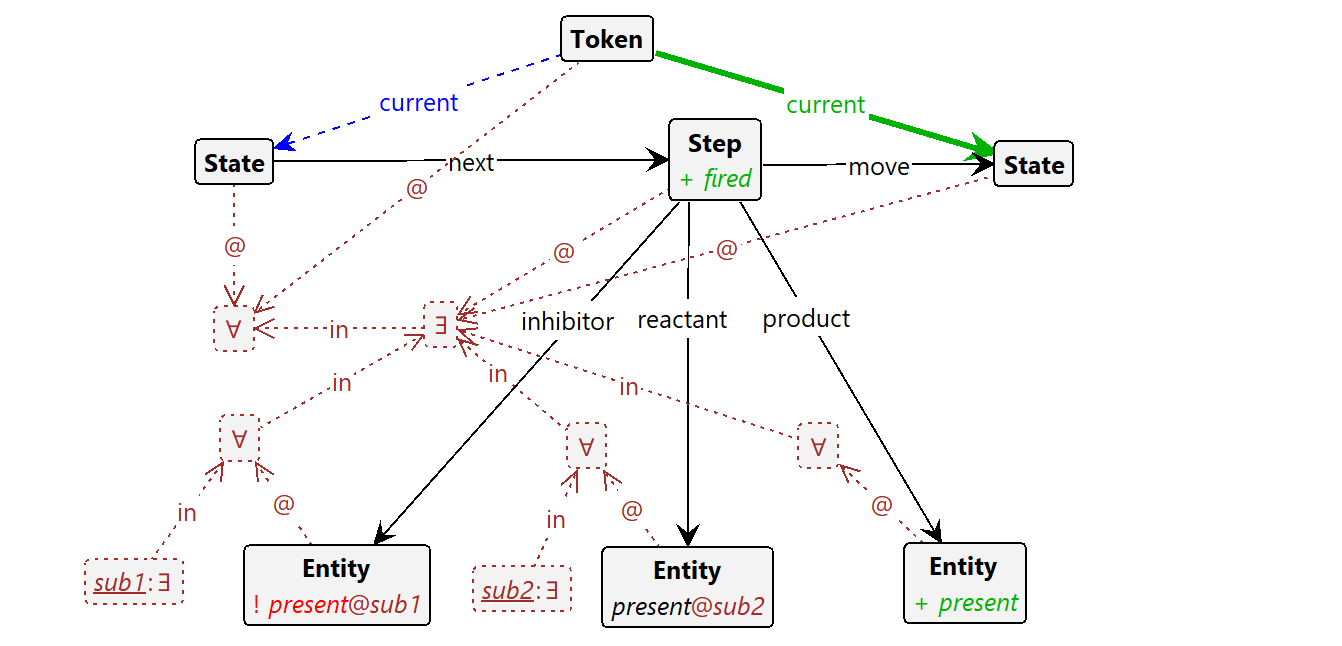
\includegraphics[scale=.2]{figs/context}
\caption{Rule for context firing}
\label{fig:context}
\end{figure}
%
\Cref{fig:context} shows the first (and most intricate) of these rules, viz.\ the one for the context firing. This is a quantified rule, which can be read as follows: \uline{For all} \State{}s with a \Token, \uline{there is} a \nextt{} \Step such that \uline{for all} \inhibitor{}s \uline{there is no} \present flag whereas \uline{for all} \reactant{}s \uline{there is} a \present flag; moreover, when the rule is applied, \uline{all} \product{}s of the selected \Step{}s receive a \present flag, the \Step{}s themselves receive a \fired flag, and all \Token{}s move to the successor \State{}s. Colour coding is used in the visual representation to distinguish the quantifier nodes $\forall$ and $\exists$ (both in purple), as well as the mandatory absence (red), deletion (blue) and creation (green) of edges and flags.\footnote{This colour coding is \GROOVE-specific and entirely separate from the problem-specific colouring of the graph nodes in Figures \ref{fig:core-type} and~\ref{fig:toy}; in fact, to avoid confusion, the problem-specific colouring is \emph{not} used in the rule view.}

To mimic the \BioResolve semantics as closely as possible, we can instruct \GROOVE to regard every pair of \contextR- and \reactR-transitions as an atomic transaction, corresponding precisely to a transition in \BioResolve (though not with the same label), and then generate the entire state space. This is achieved through a control program of the form
%
\begin{lstlisting}[keywordstyle=\bfseries,morekeywords={recipe}]
recipe fire() {
  context; react;
}
\end{lstlisting}
%
where a ``recipe'' is the keyword for a transaction wrapping the body. With this in place, the GUI-based version of \GROOVE produces the transition system displayed in \Cref{fig:toy-gts} (which can also be exported to a range of standard formats), which is easily (visually) checked to be essentially isomorphic to the one in \Cref{fig:toylts}.

\begin{figure}
\centering
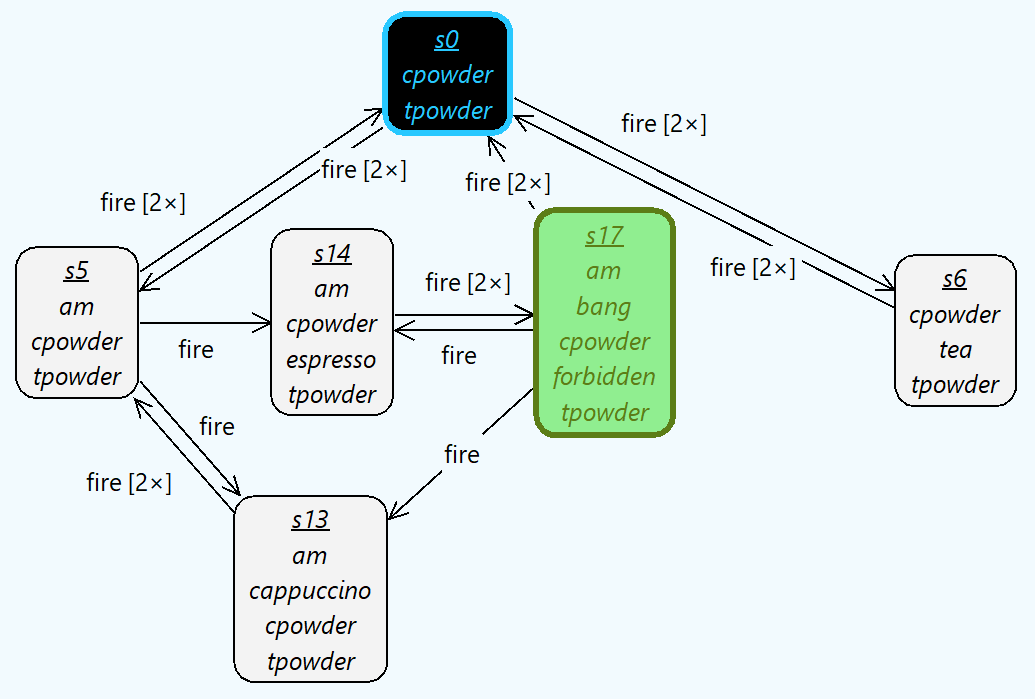
\includegraphics[scale=.2]{figs/toy-gts}
\caption{\GROOVE LTS of the toy example}
\label{fig:toy-gts}
\end{figure}

Alternatively, we can (for instance) ask \GROOVE to search the for the first reachable state in which a \Forbidden entity appears, using breadth-first search. (In fact, the state property for which \GROOVE searches is itself determined by a \emph{rule}, which in this case merely tests for the presence of a \Forbidden entity). When found, the trace to the forbidden state can be saved as a control program that drives the next stage of \GROOVE exploration. In particular, using the alternating application of the \contextR and \reactR rules (rather than the transactional variant used for \Cref{fig:toy-gts}) this control program also records the \firedR-applications that tell which \Step{}s have fired: this completely determines how the non-determinism in the context process has been resolved in order to arrive at the forbidden state. Here is the control program for the shortest trace to state \textsf{\itshape s17} in our running example:

\begin{center}
\begin{lstlisting}
context;
fired("student_2");
fired("refill_1");
react;
context;
fired("student_1");
fired("refill_0");
react;
context;
fired("refill_1");
fired("getcappuccino_1");
react;
\end{lstlisting}
\end{center}
%
Here \textsf{student\_2}, \textsf{student\_1} and \textsf{getcappucino\_1} are the \Step{}s of the \textsf{Student} process visualised in \Cref{fig:toy}; \textsf{refill\_1} and \textsf{refill\_0} are the steps of the \textsf{Refill} process given in \Cref{sec:student}.

\medskip\noindent\textbf{Build.}
%
The purpose of this phase is to build an occurrence graph that explains how \Forbidden was produced, by collecting its (transitive) dependencies~\cite{DBLP:journals/sttt/BrodoBFGMMP24}. Concretely, we record the following dependencies:
\begin{itemize}
\item From each non-initial \Entity instance to the \Rule occurrence of which it is the \product;
\item From each \Rule occurrence to all its reactant \Entity instances;
\item From each \Step occurrence to all directly preceding \Step occurrences.
\end{itemize}
%
\Cref{fig:occur-type} shows the occurrence type graph.
\begin{figure}
\centering
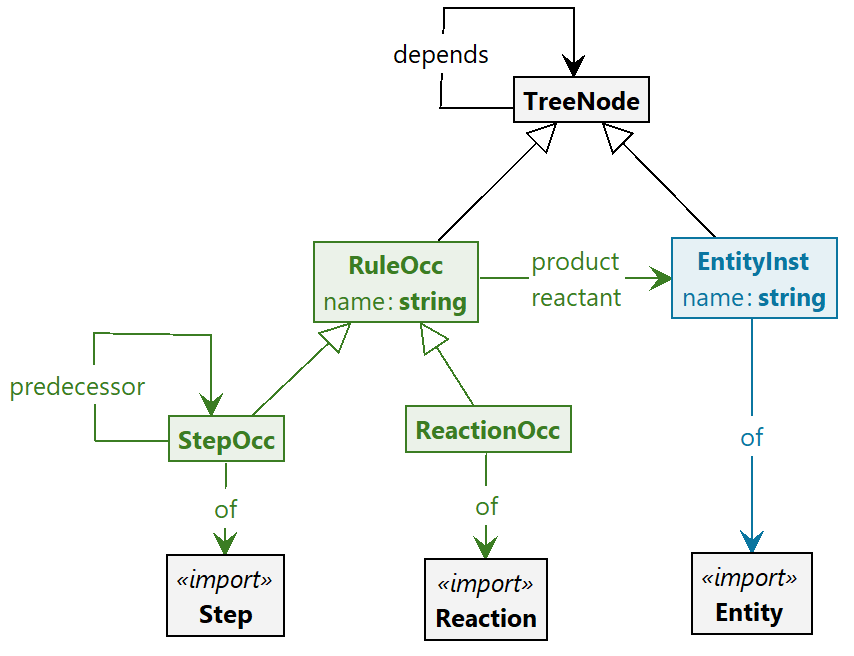
\includegraphics[scale=.2]{figs/occur-type}
\caption{Occurrence type graph}
\label{fig:occur-type}
\end{figure}
%
With respect to the slicing algorithm used in, e.g., \cite{datamod2023,DBLP:journals/nc/BrodoBF24}, the difference is that our dependencies are based on instances, and that we explicitly include the rule occurrences and their predecessors. Each of these different kinds of dependencies is visualised both through a specific edge (\product, \reactant or \predecessor) between the relevant instance- and occurrence-nodes, and (for the sake of a more uniform treatment during the next step of \emph{pruning}) through an auxiliary \depends-edge on the level of \TreeNode, of which all others are subtypes.

Note that all this is restricted to \emph{positive} dependencies. In fact, we have constructed our example so that there are no inhibitors in the \Rule{}s that fire in the trace above; if we would rely on an entity \milk that inhibits the production of \espresso, rather than on \nomilk as a reactant, the occurrence graph for \bang would not include \milk; and likewise if we would use \cappuccino as an inhibitor for \anger rather than \espresso as a reactant for it. The representation of negative dependencies is a research question in its own, and is outside the scope of this paper (although a possibility to capture negative dependencies is to focus the analysis on the Positive RS that results from the transformation defined in~\cite{DBLP:journals/sttt/BrodoBFGMMP24}).

As indicated in \Cref{fig:chain}, the occurrence graph is produced by another \GROOVE rule system, using the same start graph but driven by the control program previously created in the explore phase, which encodes (as we have seen) the trace to the undesirable state. The occurrence graph semantics consists of rules with the same names (\reactR, \contextR and \firedR), but different functionality: in particular, rather than manipulating \present flags, the \reactR rule now creates \RuleOcc- and \EntityInst-nodes together with their dependencies. This is a non-trivial procedure that in fact itself requires several successive stages. Though the details of these stages are not of sufficient interest to include in this paper, we want to point out that breaking down a single rule (\reactR, in this case) into multiple stages would seem to contradict the tenet of algebraic graph transformation that a rule embodies a single, atomic change to a graph. This contradiction is solved by relying once more on \GROOVE recipes: in the occurrence graph semantics, \reactR is actually not a rule but a recipe, defined as

\begin{center}
\begin{lstlisting}[]
recipe react() {
  entities-age;
  react-produce;
  merge;
}
\end{lstlisting}
\end{center}
%
of which the three atomic steps perform the necessary bookkeeping to correctly produce the occurrence graph.

\medskip\noindent\textbf{Prune.}
%
The occurrence graph built by the rule system described above is too large to be useful: it contains \emph{all} entity instances and rule occurrences produced by the trace, not just the dependencies of the undesired \Forbidden entity. Moreover, the entire start graph is also (still) present. Therefore, in a third phase, all redundant information is pruned. This is achieved by first marking all transitive backward dependencies, and then removing all unmarked nodes. Since this is straightforward, and of no particular interest in the context of this paper, we omit the details of the \GROOVE rule system for this phase. Its outcome for our running example is shown in \Cref{fig:toy-pruned} (where we have elided the auxiliary \depends-edges).


\begin{figure}
\centering
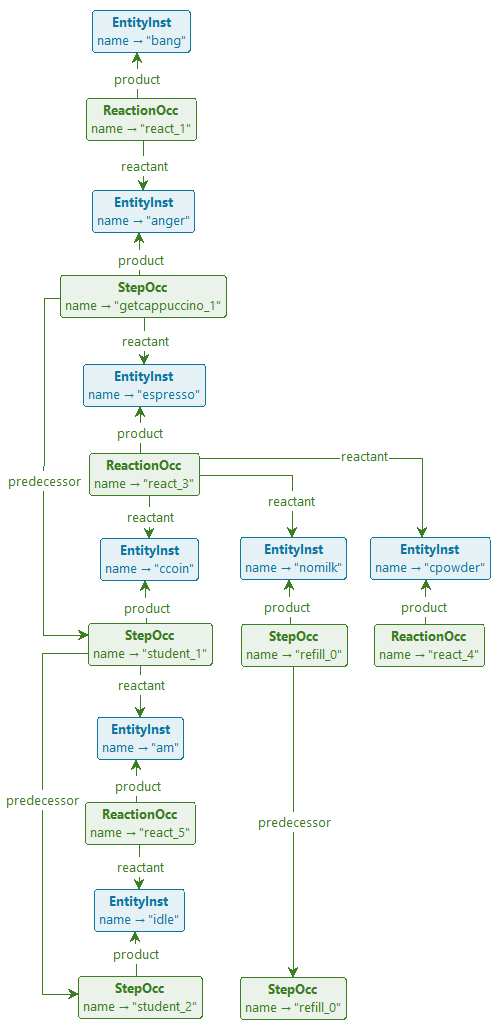
\includegraphics[width=\columnwidth]{figs/toy-pruned}
\caption{Pruned occurrence graph of the running example}
\label{fig:toy-pruned}
\end{figure}

The pruned occurrence graph visualises the causal effect chain already explained informally at the end of \Cref{sec:student}: the presence of a \ccoin, which itself depends on \am, combined with \cpowder and \nomilk causes the production of \espresso, after which the student produces \anger and then \bang, which is \Forbidden.

\begin{comment}
\begin{quote}\it Notes:
\begin{itemize}
\item Rules for implementing RS semantics
\item Conversion of a trace to a control program
\item Using recipes in the occurrence graph building
\end{itemize}
\end{quote}
\end{comment}